\documentclass[aspectratio=169]{beamer}

% ============================================
% DATABRICKS THEME - COLOR DEFINITIONS
% ============================================
\usepackage{tikz}
\usepackage{graphicx}
\usepackage{hyperref}
\usepackage{xcolor}
\usepackage{booktabs}
\usepackage{fontspec}
\usepackage{listings}

% Databricks Color Palette
\definecolor{databricksBlue}{RGB}{41, 49, 66}
\definecolor{databricksRed}{RGB}{220, 53, 69}
\definecolor{databricksYellow}{RGB}{255, 193, 7}
\definecolor{databricksGreen}{RGB}{76, 175, 80}
\definecolor{databricksGray}{RGB}{128, 128, 128}
\definecolor{databricksLightGray}{RGB}{245, 245, 245}
\definecolor{databricksWhite}{RGB}{255, 255, 255}

% ============================================
% BEAMER THEME CONFIGURATION
% ============================================
\usetheme{default}
\usecolortheme{default}

% Set colors
\setbeamercolor{structure}{fg=databricksBlue}
\setbeamercolor{frametitle}{bg=databricksBlue, fg=databricksWhite}
\setbeamercolor{title}{fg=databricksWhite}
\setbeamercolor{subtitle}{fg=databricksLightGray}
\setbeamercolor{author}{fg=databricksWhite}
\setbeamercolor{date}{fg=databricksWhite}
\setbeamercolor{institute}{fg=databricksWhite}
\setbeamercolor{background canvas}{bg=databricksWhite}
\setbeamercolor{normal text}{fg=databricksBlue}
\setbeamercolor{itemize item}{fg=databricksBlue}
\setbeamercolor{itemize subitem}{fg=databricksRed}
\setbeamercolor{itemize subsubitem}{fg=databricksGreen}
\setbeamercolor{block title}{bg=databricksBlue, fg=databricksWhite}
\setbeamercolor{block body}{bg=databricksLightGray, fg=databricksBlue}

% Itemize symbols
\setbeamertemplate{itemize item}{\textcolor{databricksBlue}{$\bullet$}}
\setbeamertemplate{itemize subitem}{\textcolor{databricksRed}{$\triangleright$}}
\setbeamertemplate{itemize subsubitem}{\textcolor{databricksGreen}{$\circ$}}

% Remove navigation symbols
\setbeamertemplate{navigation symbols}{}

% ============================================
% CUSTOM FOOTER WITH HYPERLINKS
% ============================================
\setbeamertemplate{footline}{
    \leavevmode%
    \hbox{%
        \begin{beamercolorbox}[wd=.33\paperwidth,ht=2.5ex,dp=1ex,left]{author in head/foot}%
            \usebeamerfont{author in head/foot}\hspace*{2ex}%
            \href{https://easy-ai-labs.lovable.app/}{\textcolor{databricksBlue}{Easy AI Labs}}
        \end{beamercolorbox}%
        \begin{beamercolorbox}[wd=.34\paperwidth,ht=2.5ex,dp=1ex,center]{title in head/foot}%
            \usebeamerfont{title in head/foot}%
            \href{https://www.linkedin.com/in/yashkavaiya}{\textcolor{databricksBlue}{Yash Kavaiya}}
        \end{beamercolorbox}%
        \begin{beamercolorbox}[wd=.33\paperwidth,ht=2.5ex,dp=1ex,right]{date in head/foot}%
            \usebeamerfont{date in head/foot}%
            \href{https://www.linkedin.com/company/genai-guru}{\textcolor{databricksBlue}{Gen AI Guru}}\hspace*{2ex}
            \insertframenumber{} / \inserttotalframenumber\hspace*{2ex}
        \end{beamercolorbox}%
    }%
    \vskip0pt%
}

% ============================================
% TITLE PAGE CONFIGURATION
% ============================================
\setbeamertemplate{title page}{
    \begin{tikzpicture}[remember picture,overlay]
        \fill[databricksBlue] (current page.north west) rectangle (current page.south east);
    \end{tikzpicture}
    \vfill
    \begin{center}
        {\Huge\bfseries\textcolor{databricksWhite}{\inserttitle}\par}
        \vspace{0.5cm}
        {\large\textcolor{databricksYellow}{\insertsubtitle}\par}
        \vspace{1cm}
        {\textcolor{databricksWhite}{\insertauthor}\par}
        \vspace{0.3cm}
        {\small\textcolor{databricksLightGray}{\insertdate}\par}
    \end{center}
    \vfill
}

% ============================================
% DOCUMENT INFO
% ============================================
\title{Apache Spark Fundamentals}
\subtitle{Architecture, DataFrames, Lazy Evaluation \& Practical Tasks}
\author{Yash Kavaiya}
\date{14-Day AI Challenge - Day 2}

\begin{document}

% ============================================
% TITLE SLIDE
% ============================================
\frame{\titlepage}

% ============================================
% TABLE OF CONTENTS
% ============================================
\begin{frame}{Agenda}
    \begin{columns}[T]
        \begin{column}{0.5\textwidth}
            \begin{itemize}
                \item \textcolor{databricksBlue}{\textbf{Introduction to Apache Spark}}
                \item \textcolor{databricksBlue}{\textbf{Spark Architecture Deep Dive}}
                    \begin{itemize}
                        \item Driver, Executors, Cluster Manager
                        \item DAG (Directed Acyclic Graph)
                    \end{itemize}
                \item \textcolor{databricksBlue}{\textbf{DataFrames vs RDDs}}
                    \begin{itemize}
                        \item Performance Comparison
                        \item When to Use What
                    \end{itemize}
            \end{itemize}
        \end{column}
        \begin{column}{0.5\textwidth}
            \begin{itemize}
                \item \textcolor{databricksBlue}{\textbf{Lazy Evaluation}}
                    \begin{itemize}
                        \item Transformations vs Actions
                        \item Benefits \& Optimization
                    \end{itemize}
                \item \textcolor{databricksBlue}{\textbf{Notebook Magic Commands}}
                \item \textcolor{databricksBlue}{\textbf{Practical E-Commerce Analysis}}
                    \begin{itemize}
                        \item Select, Filter, GroupBy, OrderBy
                    \end{itemize}
            \end{itemize}
        \end{column}
    \end{columns}
\end{frame}

% ============================================
% SECTION 1: INTRODUCTION TO SPARK
% ============================================
\begin{frame}{What is Apache Spark?}
    \begin{block}{Definition}
        An \textbf{open-source, distributed computing system} designed for fast, general-purpose cluster computing. Developed at UC Berkeley's AMPLab in 2009.
    \end{block}
    \vspace{0.3cm}
    \begin{columns}[T]
        \begin{column}{0.5\textwidth}
            \textcolor{databricksRed}{\textbf{MapReduce Problems:}}
            \begin{itemize}
                \item Disk I/O bottleneck
                \item Not suitable for iterative algorithms
                \item Complex programming model
            \end{itemize}
        \end{column}
        \begin{column}{0.5\textwidth}
            \textcolor{databricksGreen}{\textbf{Spark Solutions:}}
            \begin{itemize}
                \item \textbf{In-memory computing} (100x faster)
                \item Unified engine for all workloads
                \item Rich APIs (Python, Scala, Java, R)
            \end{itemize}
        \end{column}
    \end{columns}
\end{frame}

% ============================================
% SPARK ECOSYSTEM
% ============================================
\begin{frame}{Spark Ecosystem Components}
    \begin{center}
        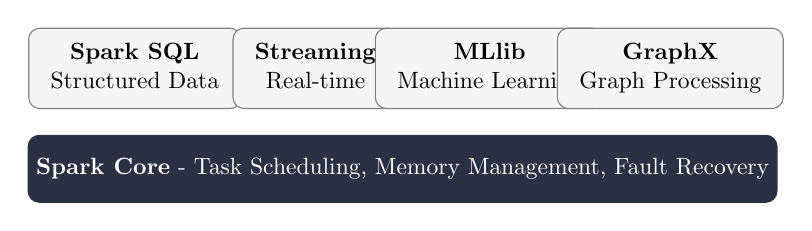
\begin{tikzpicture}[scale=0.85, every node/.style={transform shape}]
            % Core
            \node[draw=databricksBlue, fill=databricksBlue, text=databricksWhite, rounded corners, minimum width=10cm, minimum height=1cm] (core) at (0,0) {\textbf{Spark Core} - Task Scheduling, Memory Management, Fault Recovery};
            
            % Components on top
            \node[draw=databricksGray, fill=databricksLightGray, rounded corners, minimum width=2.2cm, minimum height=1.2cm] (sql) at (-4,1.5) {\begin{tabular}{c}\textbf{Spark SQL}\\Structured Data\end{tabular}};
            
            \node[draw=databricksGray, fill=databricksLightGray, rounded corners, minimum width=2.2cm, minimum height=1.2cm] (streaming) at (-1.3,1.5) {\begin{tabular}{c}\textbf{Streaming}\\Real-time\end{tabular}};
            
            \node[draw=databricksGray, fill=databricksLightGray, rounded corners, minimum width=2.2cm, minimum height=1.2cm] (mllib) at (1.3,1.5) {\begin{tabular}{c}\textbf{MLlib}\\Machine Learning\end{tabular}};
            
            \node[draw=databricksGray, fill=databricksLightGray, rounded corners, minimum width=2.2cm, minimum height=1.2cm] (graphx) at (4,1.5) {\begin{tabular}{c}\textbf{GraphX}\\Graph Processing\end{tabular}};
        \end{tikzpicture}
    \end{center}
    \vspace{0.3cm}
    \begin{alertblock}{Key Insight}
        Spark provides a \textbf{unified platform} for batch processing, streaming, SQL, ML, and graph analytics.
    \end{alertblock}
\end{frame}

% ============================================
% SPARK ARCHITECTURE
% ============================================
\begin{frame}{Spark Architecture Overview}
    \begin{center}
        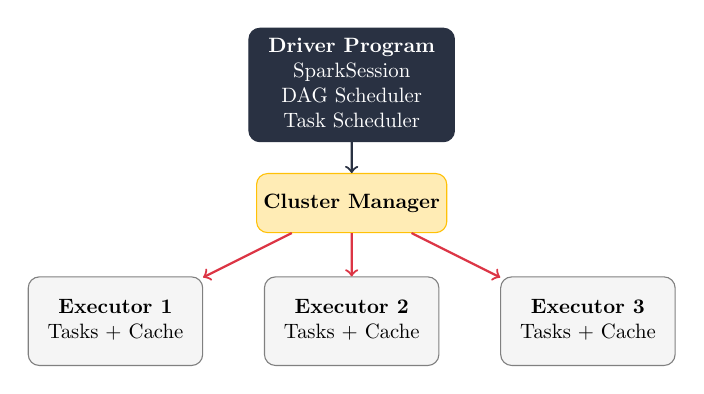
\begin{tikzpicture}[scale=0.75, every node/.style={transform shape}]
            % Driver
            \node[draw=databricksBlue, fill=databricksBlue, text=databricksWhite, rounded corners, minimum width=3cm, minimum height=1.8cm] (driver) at (0,2) {\begin{tabular}{c}\textbf{Driver Program}\\SparkSession\\DAG Scheduler\\Task Scheduler\end{tabular}};
            
            % Cluster Manager
            \node[draw=databricksYellow, fill=databricksYellow!30, rounded corners, minimum width=2.5cm, minimum height=1cm] (cm) at (0,0) {\textbf{Cluster Manager}};
            
            % Executors
            \node[draw=databricksGray, fill=databricksLightGray, rounded corners, minimum width=2.2cm, minimum height=1.5cm] (e1) at (-4,-2) {\begin{tabular}{c}\textbf{Executor 1}\\Tasks + Cache\end{tabular}};
            \node[draw=databricksGray, fill=databricksLightGray, rounded corners, minimum width=2.2cm, minimum height=1.5cm] (e2) at (0,-2) {\begin{tabular}{c}\textbf{Executor 2}\\Tasks + Cache\end{tabular}};
            \node[draw=databricksGray, fill=databricksLightGray, rounded corners, minimum width=2.2cm, minimum height=1.5cm] (e3) at (4,-2) {\begin{tabular}{c}\textbf{Executor 3}\\Tasks + Cache\end{tabular}};
            
            % Arrows
            \draw[->, thick, databricksBlue] (driver) -- (cm);
            \draw[->, thick, databricksRed] (cm) -- (e1);
            \draw[->, thick, databricksRed] (cm) -- (e2);
            \draw[->, thick, databricksRed] (cm) -- (e3);
        \end{tikzpicture}
    \end{center}
    \vspace{0.2cm}
    \begin{block}{Architecture Pattern}
        \textbf{Master-Slave} model: Driver (brain) $\rightarrow$ Cluster Manager (resources) $\rightarrow$ Executors (workers)
    \end{block}
\end{frame}

% ============================================
% DRIVER PROGRAM
% ============================================
\begin{frame}{Driver Program - The Brain}
    \begin{columns}[T]
        \begin{column}{0.5\textwidth}
            \textcolor{databricksBlue}{\textbf{Key Responsibilities:}}
            \begin{itemize}
                \item Creates \textbf{SparkSession/SparkContext}
                \item Converts user code to tasks
                \item Schedules tasks on executors
                \item Maintains metadata about RDDs
            \end{itemize}
        \end{column}
        \begin{column}{0.5\textwidth}
            \textcolor{databricksRed}{\textbf{Memory Considerations:}}
            \begin{itemize}
                \item Holds application metadata
                \item Collects results with \texttt{collect()}
                \item Broadcasts variables to executors
            \end{itemize}
            \vspace{0.3cm}
            \begin{alertblock}{Warning}
                \texttt{collect()} on large data $\Rightarrow$ \textbf{OutOfMemoryError!}
            \end{alertblock}
        \end{column}
    \end{columns}
\end{frame}

% ============================================
% EXECUTORS
% ============================================
\begin{frame}{Executors - The Workers}
    \begin{block}{Definition}
        Worker processes that execute tasks and store data. Each executor runs on a worker node in the cluster.
    \end{block}
    \vspace{0.3cm}
    \begin{columns}[T]
        \begin{column}{0.5\textwidth}
            \textcolor{databricksBlue}{\textbf{Characteristics:}}
            \begin{itemize}
                \item Launched at app start, run for lifetime
                \item Execute tasks, return results
                \item Store cached RDDs/DataFrames
                \item Multiple cores for parallel tasks
            \end{itemize}
        \end{column}
        \begin{column}{0.5\textwidth}
            \textcolor{databricksGreen}{\textbf{Memory Division:}}
            \begin{itemize}
                \item \textbf{Storage Memory:} Caching
                \item \textbf{Execution Memory:} Shuffles, joins
                \item \textbf{User Memory:} Data structures
                \item \textbf{Reserved:} 300MB fixed
            \end{itemize}
        \end{column}
    \end{columns}
\end{frame}

% ============================================
% CLUSTER MANAGERS
% ============================================
\begin{frame}{Cluster Managers}
    \begin{block}{Purpose}
        External service that manages resources across the cluster and allocates resources to applications.
    \end{block}
    \vspace{0.3cm}
    \begin{center}
        \scriptsize
        \begin{tabular}{l|ll}
            \toprule
            \textbf{Type} & \textbf{Description} & \textbf{Use Case} \\
            \midrule
            \textbf{Standalone} & Spark's built-in manager & Development, learning \\
            \textbf{YARN} & Hadoop's resource manager & Production Hadoop \\
            \textbf{Mesos} & Apache Mesos & Multi-framework \\
            \textbf{Kubernetes} & Container orchestration & Cloud-native \\
            \textbf{Local} & Single JVM & Testing \\
            \bottomrule
        \end{tabular}
    \end{center}
\end{frame}

% ============================================
% DAG
% ============================================
\begin{frame}{DAG - Directed Acyclic Graph}
    \begin{block}{Spark's Secret Weapon for Optimization}
        When you write Spark code, it builds a DAG of operations before executing.
    \end{block}
    \vspace{0.3cm}
    \begin{columns}[T]
        \begin{column}{0.5\textwidth}
            \textcolor{databricksBlue}{\textbf{DAG Properties:}}
            \begin{itemize}
                \item \textbf{Directed:} Operations flow input $\rightarrow$ output
                \item \textbf{Acyclic:} No circular dependencies
                \item \textbf{Graph:} Visual computation representation
            \end{itemize}
        \end{column}
        \begin{column}{0.5\textwidth}
            \textcolor{databricksGreen}{\textbf{Execution Flow:}}
            \begin{itemize}
                \item Build Logical Plan
                \item Optimize the Plan
                \item Create Physical Plan
                \item Divide into Stages
                \item Create Tasks
            \end{itemize}
        \end{column}
    \end{columns}
\end{frame}

% ============================================
% STAGES AND SHUFFLES
% ============================================
\begin{frame}{Stages and Shuffles}
    \begin{center}
        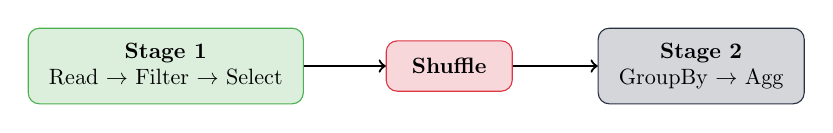
\begin{tikzpicture}[scale=0.8, every node/.style={transform shape}]
            % Stage 1
            \node[draw=databricksGreen, fill=databricksGreen!20, rounded corners, minimum width=3cm, minimum height=1.2cm] (s1) at (0,0) {\begin{tabular}{c}\textbf{Stage 1}\\Read $\rightarrow$ Filter $\rightarrow$ Select\end{tabular}};
            
            % Shuffle
            \node[draw=databricksRed, fill=databricksRed!20, rounded corners, minimum width=2cm, minimum height=0.8cm] (shuffle) at (4.5,0) {\textbf{Shuffle}};
            
            % Stage 2
            \node[draw=databricksBlue, fill=databricksBlue!20, rounded corners, minimum width=2.5cm, minimum height=1.2cm] (s2) at (8.5,0) {\begin{tabular}{c}\textbf{Stage 2}\\GroupBy $\rightarrow$ Agg\end{tabular}};
            
            \draw[->, thick] (s1) -- (shuffle);
            \draw[->, thick] (shuffle) -- (s2);
        \end{tikzpicture}
    \end{center}
    \vspace{0.3cm}
    \begin{columns}[T]
        \begin{column}{0.5\textwidth}
            \textcolor{databricksGreen}{\textbf{Narrow Transformations:}}
            \begin{itemize}
                \item One input $\rightarrow$ one output partition
                \item \texttt{map}, \texttt{filter}, \texttt{select}
                \item \textbf{No shuffle needed}
            \end{itemize}
        \end{column}
        \begin{column}{0.5\textwidth}
            \textcolor{databricksRed}{\textbf{Wide Transformations:}}
            \begin{itemize}
                \item Input $\rightarrow$ multiple output partitions
                \item \texttt{groupBy}, \texttt{reduceByKey}, \texttt{join}
                \item \textbf{Requires shuffle (expensive!)}
            \end{itemize}
        \end{column}
    \end{columns}
\end{frame}

% ============================================
% RDD
% ============================================
\begin{frame}{What is RDD?}
    \begin{block}{Resilient Distributed Dataset}
        The fundamental data structure of Spark - an immutable, distributed collection of objects.
    \end{block}
    \vspace{0.3cm}
    \begin{columns}[T]
        \begin{column}{0.5\textwidth}
            \textcolor{databricksBlue}{\textbf{Key Properties:}}
            \begin{itemize}
                \item \textbf{Resilient:} Fault-tolerant via lineage
                \item \textbf{Distributed:} Data across nodes
                \item \textbf{Dataset:} Partitioned collection
            \end{itemize}
        \end{column}
        \begin{column}{0.5\textwidth}
            \textcolor{databricksGreen}{\textbf{Creating RDDs:}}
            \begin{itemize}
                \item From collection: \texttt{parallelize()}
                \item From file: \texttt{textFile()}
                \item From another RDD: \texttt{map()}
            \end{itemize}
        \end{column}
    \end{columns}
    \vspace{0.3cm}
    \begin{exampleblock}{RDD Lineage}
        RDDs track their transformation history, enabling automatic recomputation of lost partitions.
    \end{exampleblock}
\end{frame}

% ============================================
% DATAFRAME
% ============================================
\begin{frame}{What is DataFrame?}
    \begin{block}{Definition}
        A distributed collection of data organized into named columns, similar to a database table or pandas DataFrame.
    \end{block}
    \vspace{0.3cm}
    \begin{columns}[T]
        \begin{column}{0.5\textwidth}
            \textcolor{databricksBlue}{\textbf{Key Features:}}
            \begin{itemize}
                \item Has defined \textbf{schema}
                \item \textbf{Catalyst} optimizer
                \item \textbf{Tungsten} execution engine
                \item SQL + DSL APIs
            \end{itemize}
        \end{column}
        \begin{column}{0.5\textwidth}
            \textcolor{databricksGreen}{\textbf{Creating DataFrames:}}
            \begin{itemize}
                \item \texttt{spark.read.csv()}
                \item \texttt{spark.read.json()}
                \item \texttt{spark.read.parquet()}
                \item \texttt{spark.createDataFrame()}
            \end{itemize}
        \end{column}
    \end{columns}
\end{frame}

% ============================================
% RDD VS DATAFRAME COMPARISON
% ============================================
\begin{frame}{RDD vs DataFrame Comparison}
    \begin{center}
        \scriptsize
        \begin{tabular}{l|cc}
            \toprule
            \textbf{Aspect} & \textbf{RDD} & \textbf{DataFrame} \\
            \midrule
            Abstraction & Low-level & High-level \\
            Schema & No schema & Has schema \\
            Optimization & No automatic & Catalyst + Tungsten \\
            Performance & Slower & \textcolor{databricksGreen}{\textbf{Faster}} \\
            Memory Usage & Higher (Java objects) & Lower (off-heap) \\
            APIs & Functional transformations & SQL + DSL \\
            Use Case & Unstructured data & Structured data \\
            \bottomrule
        \end{tabular}
    \end{center}
    \vspace{0.3cm}
    \begin{block}{Recommendation}
        \textbf{Use DataFrames} for most use cases. Use RDDs only when you need fine-grained control over physical execution or work with unstructured data.
    \end{block}
\end{frame}

% ============================================
% CATALYST AND TUNGSTEN
% ============================================
\begin{frame}{Why DataFrames are Faster}
    \begin{columns}[T]
        \begin{column}{0.5\textwidth}
            \textcolor{databricksBlue}{\textbf{Catalyst Optimizer:}}
            \begin{itemize}
                \item Analyzes query plans
                \item Applies optimizations:
                    \begin{itemize}
                        \item Predicate pushdown
                        \item Column pruning
                        \item Constant folding
                    \end{itemize}
                \item Generates optimized execution
            \end{itemize}
        \end{column}
        \begin{column}{0.5\textwidth}
            \textcolor{databricksGreen}{\textbf{Tungsten Engine:}}
            \begin{itemize}
                \item Off-heap memory management
                \item Avoids JVM garbage collection
                \item Cache-aware computation
                \item Runtime code generation
                \item Columnar storage format
            \end{itemize}
        \end{column}
    \end{columns}
    \vspace{0.3cm}
    \begin{alertblock}{Performance Gain}
        DataFrame operations can be \textbf{10-100x faster} than equivalent RDD operations!
    \end{alertblock}
\end{frame}

% ============================================
% LAZY EVALUATION
% ============================================
\begin{frame}{Lazy Evaluation}
    \begin{block}{Definition}
        Transformations are not executed immediately. Spark records them in a DAG and executes only when an action is called.
    \end{block}
    \vspace{0.3cm}
    \begin{center}
        \textit{Think of it like a recipe book:}\\
        \textbf{Transformations} = Writing recipe steps (no cooking)\\
        \textbf{Actions} = Actually cooking the dish (execution)
    \end{center}
    \vspace{0.3cm}
    \begin{exampleblock}{Example}
        \texttt{df.filter(...).select(...).groupBy(...)} $\rightarrow$ \textbf{Not executed yet!}\\
        \texttt{df.count()} $\rightarrow$ \textbf{NOW everything executes!}
    \end{exampleblock}
\end{frame}

% ============================================
% TRANSFORMATIONS VS ACTIONS
% ============================================
\begin{frame}{Transformations vs Actions}
    \begin{columns}[T]
        \begin{column}{0.5\textwidth}
            \textcolor{databricksBlue}{\textbf{Transformations (Lazy):}}
            \begin{itemize}
                \item \texttt{select()}
                \item \texttt{filter()} / \texttt{where()}
                \item \texttt{map()} / \texttt{flatMap()}
                \item \texttt{groupBy()}
                \item \texttt{orderBy()} / \texttt{sort()}
                \item \texttt{join()} / \texttt{union()}
                \item \texttt{withColumn()} / \texttt{drop()}
            \end{itemize}
        \end{column}
        \begin{column}{0.5\textwidth}
            \textcolor{databricksRed}{\textbf{Actions (Trigger Execution):}}
            \begin{itemize}
                \item \texttt{show()}
                \item \texttt{count()}
                \item \texttt{collect()}
                \item \texttt{first()} / \texttt{take(n)}
                \item \texttt{reduce()}
                \item \texttt{foreach()}
                \item \texttt{write.save()}
            \end{itemize}
        \end{column}
    \end{columns}
\end{frame}

% ============================================
% BENEFITS OF LAZY EVALUATION
% ============================================
\begin{frame}{Benefits of Lazy Evaluation}
    \begin{columns}[T]
        \begin{column}{0.5\textwidth}
            \textcolor{databricksBlue}{\textbf{Query Optimization:}}
            \begin{itemize}
                \item Predicate pushdown
                \item Column pruning
                \item Combined operations
            \end{itemize}
            \vspace{0.3cm}
            \textcolor{databricksGreen}{\textbf{Fault Tolerance:}}
            \begin{itemize}
                \item Lineage enables recomputation
                \item Lost partitions recovered automatically
            \end{itemize}
        \end{column}
        \begin{column}{0.5\textwidth}
            \textcolor{databricksRed}{\textbf{Memory Efficiency:}}
            \begin{itemize}
                \item No intermediate materialization
                \item Stream processing through pipeline
            \end{itemize}
            \vspace{0.3cm}
            \textcolor{databricksYellow}{\textbf{Pipelining:}}
            \begin{itemize}
                \item Narrow transformations combined
                \item Single pass through data
            \end{itemize}
        \end{column}
    \end{columns}
    \vspace{0.3cm}
    \begin{alertblock}{Common Pitfall}
        Multiple actions re-execute entire DAG! Use \texttt{.cache()} for reused DataFrames.
    \end{alertblock}
\end{frame}

% ============================================
% MAGIC COMMANDS
% ============================================
\begin{frame}{Notebook Magic Commands}
    \begin{center}
        \scriptsize
        \begin{tabular}{l|ll}
            \toprule
            \textbf{Command} & \textbf{Description} & \textbf{Example} \\
            \midrule
            \texttt{\%python} & Execute Python code & Default in notebooks \\
            \texttt{\%sql} & Execute SQL query & \texttt{\%sql SELECT * FROM table} \\
            \texttt{\%scala} & Execute Scala code & Performance-critical code \\
            \texttt{\%r} & Execute R code & Statistical analysis \\
            \texttt{\%fs} & File system operations & \texttt{\%fs ls /data/} \\
            \texttt{\%sh} & Shell commands & \texttt{\%sh pip install pandas} \\
            \texttt{\%md} & Markdown rendering & Documentation \\
            \texttt{\%run} & Run another notebook & \texttt{\%run ./utilities} \\
            \bottomrule
        \end{tabular}
    \end{center}
    \vspace{0.3cm}
    \begin{block}{Key Feature}
        Seamlessly switch between languages in the same notebook for maximum flexibility!
    \end{block}
\end{frame}

% ============================================
% PRACTICAL TASKS INTRO
% ============================================
\begin{frame}{Practical Tasks: E-Commerce Analysis}
    \begin{block}{Objective}
        Apply Spark DataFrame operations to analyze e-commerce sales data.
    \end{block}
    \vspace{0.3cm}
    \begin{enumerate}
        \item \textcolor{databricksBlue}{\textbf{Task 1:}} Upload Sample E-Commerce CSV
        \item \textcolor{databricksBlue}{\textbf{Task 2:}} Read Data into DataFrame
        \item \textcolor{databricksBlue}{\textbf{Task 3:}} Basic DataFrame Operations
            \begin{itemize}
                \item SELECT - Choosing columns
                \item FILTER - Filtering rows
                \item GROUPBY - Aggregating data
                \item ORDERBY - Sorting results
            \end{itemize}
        \item \textcolor{databricksBlue}{\textbf{Task 4:}} Export Results
    \end{enumerate}
\end{frame}

% ============================================
% SELECT OPERATION
% ============================================
\begin{frame}{SELECT - Choosing Columns}
    \begin{block}{Purpose}
        Extract specific columns from a DataFrame.
    \end{block}
    \vspace{0.3cm}
    \begin{columns}[T]
        \begin{column}{0.5\textwidth}
            \textcolor{databricksBlue}{\textbf{Methods:}}
            \begin{itemize}
                \item String names: \texttt{df.select("col1", "col2")}
                \item Using \texttt{col()}: \texttt{df.select(col("col1"))}
                \item DataFrame ref: \texttt{df.select(df.col1)}
            \end{itemize}
        \end{column}
        \begin{column}{0.5\textwidth}
            \textcolor{databricksGreen}{\textbf{With Transformations:}}
            \begin{itemize}
                \item Alias: \texttt{col("a").alias("new\_name")}
                \item Expression: \texttt{selectExpr("a * 2")}
            \end{itemize}
        \end{column}
    \end{columns}
    \vspace{0.3cm}
    \begin{exampleblock}{Example}
        \texttt{df.select("order\_id", "product\_name", "total\_amount")}
    \end{exampleblock}
\end{frame}

% ============================================
% FILTER OPERATION
% ============================================
\begin{frame}{FILTER / WHERE - Filtering Rows}
    \begin{block}{Purpose}
        Keep only rows that satisfy certain conditions.
    \end{block}
    \vspace{0.2cm}
    \begin{center}
        \scriptsize
        \begin{tabular}{l|ll}
            \toprule
            \textbf{Operation} & \textbf{Syntax} & \textbf{Example} \\
            \midrule
            Equals & \texttt{==} & \texttt{col("city") == "NYC"} \\
            Not equals & \texttt{!=} & \texttt{col("city") != "NYC"} \\
            Greater/Less & \texttt{>}, \texttt{<}, \texttt{>=}, \texttt{<=} & \texttt{col("amount") > 100} \\
            AND & \texttt{\&} & \texttt{(cond1) \& (cond2)} \\
            OR & \texttt{|} & \texttt{(cond1) | (cond2)} \\
            IN list & \texttt{.isin()} & \texttt{col("city").isin(["A","B"])} \\
            LIKE & \texttt{.like()} & \texttt{col("name").like("\%Pro\%")} \\
            \bottomrule
        \end{tabular}
    \end{center}
\end{frame}

% ============================================
% GROUPBY OPERATION
% ============================================
\begin{frame}{GROUPBY - Aggregating Data}
    \begin{block}{Purpose}
        Group rows by column values and perform aggregate calculations.
    \end{block}
    \vspace{0.2cm}
    \begin{columns}[T]
        \begin{column}{0.5\textwidth}
            \textcolor{databricksBlue}{\textbf{Aggregation Functions:}}
            \begin{itemize}
                \item \texttt{count()} - Count rows
                \item \texttt{sum()} - Sum values
                \item \texttt{avg()} / \texttt{mean()} - Average
                \item \texttt{min()} / \texttt{max()} - Min/Max
                \item \texttt{countDistinct()} - Unique count
            \end{itemize}
        \end{column}
        \begin{column}{0.5\textwidth}
            \textcolor{databricksGreen}{\textbf{Example:}}
            \begin{itemize}
                \item \texttt{df.groupBy("category")}
                \item \texttt{.agg(}
                \item \texttt{~~count("*").alias("orders"),}
                \item \texttt{~~sum("amount").alias("total")}
                \item \texttt{)}
            \end{itemize}
        \end{column}
    \end{columns}
\end{frame}

% ============================================
% ORDERBY OPERATION
% ============================================
\begin{frame}{ORDERBY / SORT - Sorting Data}
    \begin{block}{Purpose}
        Sort rows by one or more columns.
    \end{block}
    \vspace{0.3cm}
    \begin{columns}[T]
        \begin{column}{0.5\textwidth}
            \textcolor{databricksBlue}{\textbf{Ascending (Default):}}
            \begin{itemize}
                \item \texttt{df.orderBy("column")}
                \item \texttt{df.orderBy(col("a").asc())}
            \end{itemize}
        \end{column}
        \begin{column}{0.5\textwidth}
            \textcolor{databricksRed}{\textbf{Descending:}}
            \begin{itemize}
                \item \texttt{df.orderBy(col("a").desc())}
                \item \texttt{df.orderBy(desc("a"))}
            \end{itemize}
        \end{column}
    \end{columns}
    \vspace{0.3cm}
    \begin{exampleblock}{Multiple Columns}
        \texttt{df.orderBy(col("category").asc(), col("amount").desc())}
    \end{exampleblock}
\end{frame}

% ============================================
% EXPORT RESULTS
% ============================================
\begin{frame}{Exporting Results}
    \begin{center}
        \scriptsize
        \begin{tabular}{l|l}
            \toprule
            \textbf{Format} & \textbf{Command} \\
            \midrule
            CSV & \texttt{df.write.mode("overwrite").csv("/output")} \\
            Single CSV & \texttt{df.coalesce(1).write.csv("/output")} \\
            Parquet & \texttt{df.write.parquet("/output")} \\
            JSON & \texttt{df.write.json("/output")} \\
            Table & \texttt{df.write.saveAsTable("db.table")} \\
            Partitioned & \texttt{df.write.partitionBy("col").parquet()} \\
            \bottomrule
        \end{tabular}
    \end{center}
    \vspace{0.3cm}
    \begin{block}{Write Modes}
        \textbf{overwrite} - Replace $\bullet$ \textbf{append} - Add $\bullet$ \textbf{ignore} - Skip if exists $\bullet$ \textbf{error} - Fail if exists
    \end{block}
    \vspace{0.2cm}
    \begin{alertblock}{Recommendation}
        Use \textbf{Parquet} for big data (columnar, efficient). Use CSV for interoperability.
    \end{alertblock}
\end{frame}

% ============================================
% KEY TAKEAWAYS
% ============================================
\begin{frame}{Key Takeaways}
    \begin{columns}[T]
        \begin{column}{0.5\textwidth}
            \begin{block}{Architecture}
                \begin{itemize}
                    \item Driver = Brain (scheduling)
                    \item Executors = Workers (execution)
                    \item DAG = Optimization graph
                    \item Avoid shuffles when possible
                \end{itemize}
            \end{block}
        \end{column}
        \begin{column}{0.5\textwidth}
            \begin{alertblock}{Best Practices}
                \begin{itemize}
                    \item Prefer DataFrames over RDDs
                    \item Cache reused DataFrames
                    \item Use Parquet for storage
                    \item Watch out for \texttt{collect()}
                \end{itemize}
            \end{alertblock}
        \end{column}
    \end{columns}
    \vspace{0.5cm}
    \begin{center}
        \Large\textcolor{databricksBlue}{\textbf{Spark = In-memory + DAG optimization + Unified platform}}
    \end{center}
\end{frame}

% ============================================
% THANK YOU SLIDE
% ============================================
\begin{frame}
    \begin{tikzpicture}[remember picture,overlay]
        \fill[databricksBlue] (current page.north west) rectangle (current page.south east);
    \end{tikzpicture}
    \begin{center}
        \vspace{2cm}
        {\Huge\bfseries\textcolor{databricksWhite}{Thank You!}\par}
        \vspace{1cm}
        {\large\textcolor{databricksYellow}{Questions?}\par}
        \vspace{1.5cm}
        {\textcolor{databricksWhite}{Connect with me:}\par}
        \vspace{0.3cm}
        {\href{https://www.linkedin.com/in/yashkavaiya}{\textcolor{databricksLightGray}{linkedin.com/in/yashkavaiya}}\par}
        \vspace{0.3cm}
        {\href{https://www.linkedin.com/company/genai-guru}{\textcolor{databricksLightGray}{Gen AI Guru}}\par}
    \end{center}
\end{frame}

\end{document}
